\documentclass[conference]{IEEEtran}

\IEEEoverridecommandlockouts

\usepackage{cite}
\usepackage{amsmath,amssymb,amsfonts}
\usepackage{algorithmic}
\usepackage{graphicx}
\usepackage{textcomp}
\usepackage{xcolor}

\def\BibTeX{{\rm B\kern-.05em{\sc i\kern-.025em b}\kern-.08em
    T\kern-.1667em\lower.7ex\hbox{E}\kern-.125emX}}

\begin{document}

\title{Sequence Alignment and Parallel Programming}

\author{\IEEEauthorblockN{1\textsuperscript{st} Daniel Vali}
\and
\IEEEauthorblockN{2\textsuperscript{nd} Austin Traub}
\and
\IEEEauthorblockN{3\textsuperscript{rd} Tony Pham}
}

\maketitle

% \begin{abstract}
% \end{abstract}

\section{Introduction}
The purpose of this project is to explore the algorithms and related parallel programming techniques used in sequence alignment. Sequence alignment is a process in bioinformatics whereby DNA, RNA, or protein is aligned in way that produces an optimal match between the residues of the molecules being aligned. DNA and RNA are made of nucleotides, and proteins are made of amino acids. Nucleotides and amino acids are represented as letters, and it is the sequences of those letters that are being aligned.

Sequence alignment is typically used to study the functions of biological sequences. Similarity between two biological sequences usually indicate that those sequences perform the same function. Thereby, sequence alignment is a highly useful process when it comes to studying this.

There are two main types of sequence alignments: pairwise alignment and multiple sequence alignment \cite{chaudhary_liu_matta_yang_2005}. In a pairwise alignment, two sequences are compared and aligned. In a multiple sequence alignment, multiple sequences are aligned. This project will focus on algorithms for pairwise alignment. The typical application of pairwise alignment is to allow users to search a database for sequences similar to a specified input sequence. The input sequence is compared pairwise to each sequence in the database and the best matches are returned.

Alignments can be categorized further as either global or local. A global alignment is one that finds the best alignment for the entire sequence from beginning to end \cite{global_alignment}. This is useful for comparing closely related sequences. A local alignment is one that finds similarities in only local regions of the sequences \cite{global_alignment}. This is useful for when maybe only certain regions of the sequences being compared are similar. The project will look at algorithms for both global and local alignments.

What makes the sequence alignment problem difficult is the size of the sequences usually being compared. The typical size of a DNA sequence string in FASTA format, for example, can range from 40KB to 60KB \cite{naveed_siddiqui_ahmed}. Using a sequence alignment algorithm such as the Needleman-Wunsch Algorithm, which runs in O(MN), can take some time. In addition, doing this many times over while searching a database makes this process impractical. That is why it is important to look into ways in which sequence alignment could be parallelized.

The following is an example sequence alignment for the sequences TCGATA and AGATC:\\

\quad TCGATA

\quad –AGATC\\
 
The dash before the letter A in the second sequence in the alignment represents a gap. Gaps are indicative of insertions or deletions. Sequences may have been the same at some point in time and ended up diverging through mutations involving substitutions, insertions, or deletions \cite{settles_2008}. For example, the second sequence above could have undergone a mutation where T (the first letter) was deleted and C (the second letter) was substituted with an A.

Another possible alignment for the sequences above is as follows:\\

\quad TCGATA

\quad A–GATC\\

This example indicates that, in the second sequence, a mutation could have cause T (the first letter) to be substituted with A and C (the second letter) to be deleted. To determine which alignment is best, algorithms use a scoring system to assign a score to each possible alignment. Usually, the alignment with the highest score is the optimal alignment.

The existing algorithms for sequence alignment fall into three categories: dynamic programming based, heuristic-based, or a mixture of the two \cite{chaudhary_liu_matta_yang_2005}. The dynamic programming based algorithms breaks the problem into subproblems and finds a solution using the bottom up approach. In order words, the optimal alignments for the subsequences are found, and those are used to find optimal alignment for the overall sequences. The dynamic programming based solutions are computationally demanding, making them impractical when dealing with a great number of sequences \cite{chaudhary_liu_matta_yang_2005}. As a result, heuristic approaches are typically used to approximate the optimal alignment. These heuristic solutions typically use dynamic programming for only a portion of the sequence while using approximations to make the search space more manageable. The result is a faster and more efficient algorithm.

The focus of the project is to only explore existing sequential and concurrent algorithms for sequence alignment based on dynamic programming.

\section{Goals}
As stated before, the goal of this project is the explore existing sequential and concurrent algorithms for sequence alignment based on dynamic programming. We will attempt to improve parallelization of these algorithms through experimentation.

\section{Existing Algorithms}
The following section presents some dynamic programming based algorithms for sequence alignment. The Needleman-Wunsch algorithm is used to find global alignments. The Smith-Waterman algorithm is used to find local alignments. And the Hirschberg algorithm is a space efficient modification of the Needleman-Wunsch algorithm.

\subsection{Needleman-Wunsch}
The Needleman-Wunsch algorithm uses dynamic programming to find the optimal global alignment between two sequences \cite{vladimir}. It finds the optimal alignment across the entire sequence. The algorithm is based on the idea that the overall optimal alignment of two sequences can be determined through determining the optimal alignments of their subsequences and building up from there. All possible alignments of the two sequences are determined, and a score is given to each to rank it. The alignment with the highest score is the most optimal one.

The algorithm involves the use of two matrices: the score matrix and the traceback matrix. It can be broken down into three main parts: the initialization of the two matrices, the calculating of the scores and directions in the two matrices, and using the traceback matrix to determine the optimal alignment.

The score matrix is used to store the score for each alignment. The traceback matrix is used to store the direction from which each score came from. Each score in the score matrix is calculated based on a previously calculated neighboring score. The directions in the traceback matrix are used to trace and determine the highest scoring alignment. Fig.~\ref{1} is an example score matrix, and Fig.~\ref{2} is its corresponding traceback matrix.

\begin{figure}[htbp]
\centerline{\scalebox{.75}{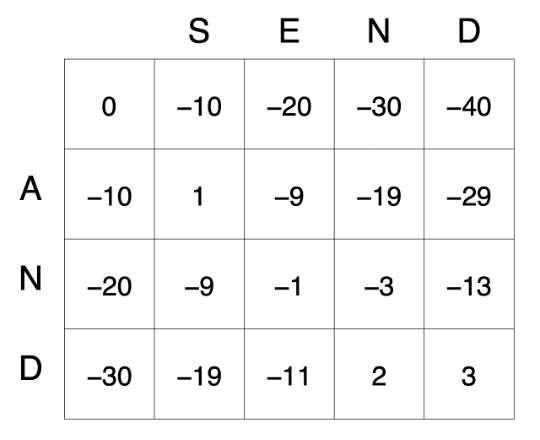
\includegraphics{Figures/1.png}}}
\caption{Example score matrix. \cite{vladimir}}
\label{1}
\end{figure}

\begin{figure}[htbp]
\centerline{\scalebox{.72}{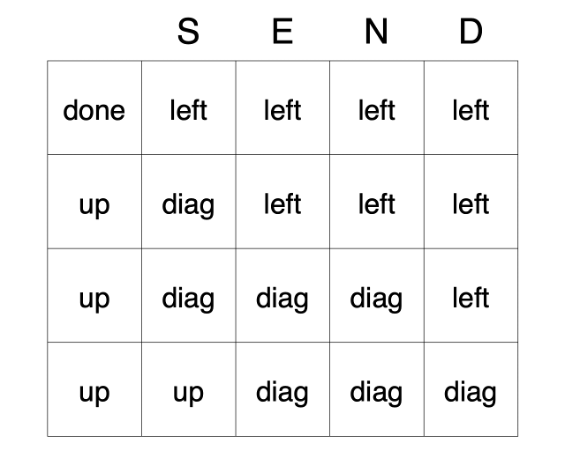
\includegraphics{Figures/2.png}}}
\caption{Example traceback matrix. \cite{vladimir}}
\label{2}
\end{figure}

A scoring scheme needs to be picked to help calculate the scores. A basic example scheme is to use +1 for a match, -1 for a mismatch, and 0 for a gap. A match occurs when two letters match. A mismatch is when the letters do not match. And a gap is where the letter from one sequence is lined up with a gap, corresponding to an insertion/deletion. Inserting a gap into a sequence shifts it, causing a letter from the other sequence to match with the gap.

A substitution matrix can also be used to define the scoring scheme more thoroughly. Using a substitution matrix, different matches/mismatches could be assigned different substitution scores. For example, a C-C match could be assigned a +1 while a T-T match could be assigned a +2. Below in Fig.~\ref{3} is an example substitution matrix. Here, all the matches are assigned +1 while all the mismatches are assigned -1. For example, the value 1 in row 2 column 2 indicates that a C-C match should have a substitution score of 1.

\begin{figure}[htbp]
\centerline{\scalebox{.72}{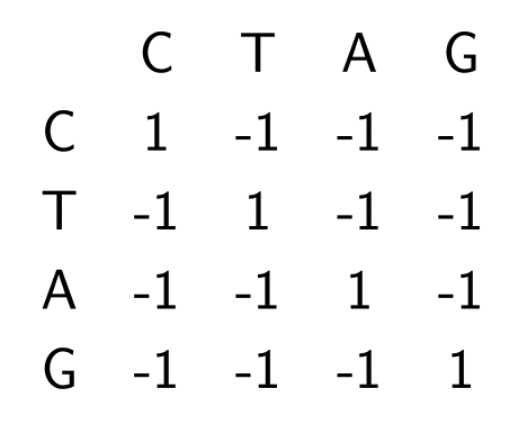
\includegraphics{Figures/3.png}}}
\caption{Example substitution matrix. \cite{vladimir}}
\label{3}
\end{figure}

To determine the score for a cell in the score matrix, the scores of the neighboring cells to the left, above, or on the top left of the current cell are taken into account. The subscore of the current cell, determined by the scoring scheme, is added to the score of each of those neighboring cells individually. The highest result out of the three is chosen as the score for the current cell. Going to the cell on the left means adding a gap to the letter on the sequence placed on the left side of the matrix. The gap penalty should be added here. Going to the cell above means adding a gap to the letter on the sequence at the top of the matrix. The gap penalty should be added here in this case. Going diagonally to the top left means that a gap was not added. Here, the match score should be added for a match, and the mismatch score should be added for a mismatch. The scoring system is represented by the recursive relation in Fig.~\ref{4}, where \textit{s(i, j)} is the substitution score and \textit{g} is the gap penalty. Fig.~\ref{5} demonstrates this relation visually on a score matrix.

\begin{figure}[htbp]
\centerline{\scalebox{.72}{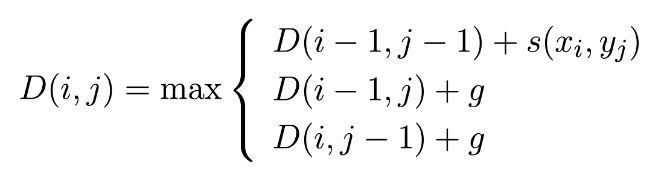
\includegraphics{Figures/4.png}}}
\caption{Recursive relation to determine the score. \cite{vladimir}}
\label{4}
\end{figure}

\begin{figure}[htbp]
\centerline{\scalebox{.72}{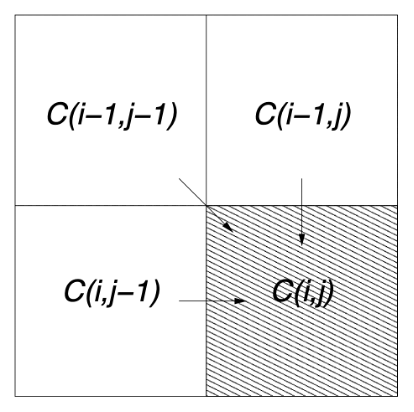
\includegraphics{Figures/5.png}}}
\caption{Determining the score on the matrix. \cite{vladimir}}
\label{5}
\end{figure}

The directions in the traceback matrix are either Left, Up, or Diagonal (for top left). The direction for each cell depends on which of the three neighboring cells was used to determine the final score for it. For example, if the final and highest score for a cell in a score matrix was calculated using the cell above it, the corresponding cell in the traceback matrix would have the value U for Up.

To demonstrate, in the score matrix below in Fig.~\ref{6}, the score for row 2 column 2 (A-A) is determined to be 2. This matrix uses -2 for the gap penalty, -3 for a mismatch, and 2 for a match. Starting at row 2 column 2, going left to row 2 column 1 means adding a gap to the sequence on the left side of the matrix. The gap penalty is -2, so the total score for going left is the sum of the left cell and the gap penalty. That is, -2 + -2 = -4. Similarly, going up to row 1 column 2 means adding a gap to the sequence at the top of the matrix. The total score here is also -2 + -2 = -4. Lastly, going diagonally to row 1 column 1 means not adding a gap. The current cell is a match since it represents the pair A-A; both the letters corresponding to the row and column of the cell are A’s. The score for a match is 2. Accordingly, the total score here is 0 + 2 = 2. Out of the three scores calculated, 2 is the highest, so it is chosen as the final score for the cell. Since the max score is calculated using the top left diagonal neighboring cell’s score, we set the corresponding cell’s value in the traceback matrix to D for diagonal. That is, we set the value of row 2 column 2 of the traceback matrix to D.

\begin{figure}[htbp]
\centerline{\scalebox{.72}{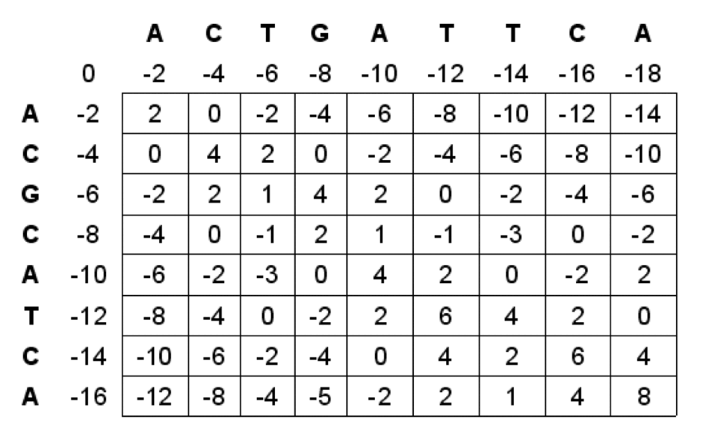
\includegraphics{Figures/6.png}}}
\caption{Another example score matrix. \cite{musso}}
\label{6}
\end{figure}

The scoring matrix is initialized by setting the top uppermost leftmost cell to 0. The gap penalty is then added incrementally both along the first row and first column. For example, in Fig.~\ref{6}, where the gap penalty is -2, the scores along the first row are 0, -2, -4, -6, -8, and so on. The scores along the first column are the same. These scores indicate the overall score for appending gaps to the beginning of each sequence. For instance, adding two gaps to the beginning of the left sequence above produces -{}-ACGCATCA. The corresponding score for this alignment is -4 since row 3 column 1 is -4.

Once all of the scores in the score matrix and the directions in the traceback matrix have been determined, the traceback matrix is used to produce the most optimal alignment between the two sequences. The traceback begins at the bottommost rightmost cell. The trace then moves either left, up, or diagonally from that point on. Movement is based on the direction stored in the traceback matrix. Moving left means adding a gap to the sequence on the left of the matrix. Moving up means adding a gap to the sequence at the top of the matrix. And moving diagonally means that the two letters for that cell are aligned and no gap is to be added. The traceback ends when the topmost leftmost cell is reached. Fig.~\ref{7} shows an example traceback matrix and its final path. The corresponding optimal alignment for the sequences SEND and AND is as follows:\\
 
\quad SEND

\quad A–ND

\begin{figure}[htbp]
\centerline{\scalebox{.7}{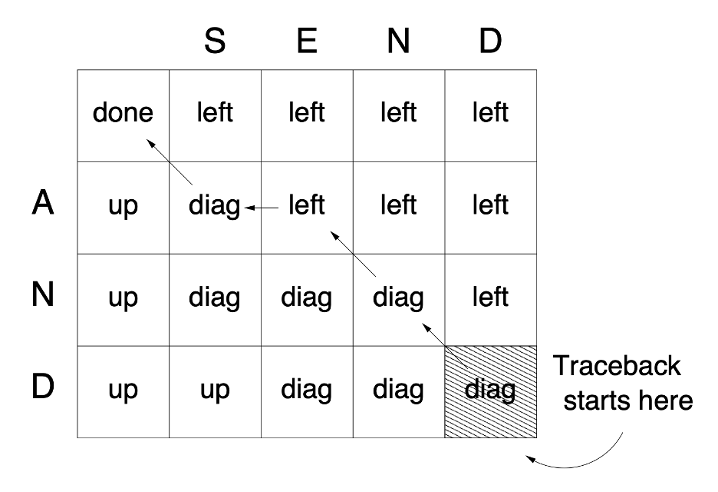
\includegraphics{Figures/7.png}}}
\caption{Another example traceback matrix. \cite{vladimir}}
\label{7}
\end{figure}

\subsection{Parallel Version of Needleman-Wunsch}

Naveed, Siddiqui, and Ahmed describes a method for parallelizing the Needleman-Wunsch algorithm \cite{naveed_siddiqui_ahmed}. This method involves two parts: the parallel initialization of the matrices used in the algorithm and the parallel calculation of the scores and directions that fill the matrices.

The score and traceback matrices each can be initialized by two separate threads. One thread can set the initial row column values (-1, -2, -3, … or Left) while the other thread can set the initial first column values (-1, -2, -3, … or Up). If the sequences are stored in the matrices as headers, they also can be stored in a similar parallel manner. One thread sets the first sequence across the top and the other sets the second sequence along the side.

As for the calculating the scores, the scores can be calculated anti-diagonally. This way, the calculations can be parallelized within each anti-diagonal. The scores in the first anti-diagonal are calculated first, then the second, the third, and so on. Fig.~\ref{8} below shows the anti-diagonals used in this technique. Calculating the scores in an anti-diagonal order is possible since each score is determined based on the cells left, above, or top left of it. The scores for the left, top, and top left cells for each cell will be already determined by the time we attempt to fill in the next anti-diagonal.

In Fig.~\ref{8} below, row 2 column 2 would be calculated first. Then row 2 column 3 and row 3 column 2 would be calculated next in parallel. Here, one thread can be used to calculate row 2 column 3 and another can be used to calculate row 3 column 2. The next calculations are row 2 column 4, row 3 column 3, and row 4 column 2 together in parallel. This pattern continues until the matrix is completely filled in.

\begin{figure}[htbp]
\centerline{\scalebox{.68}{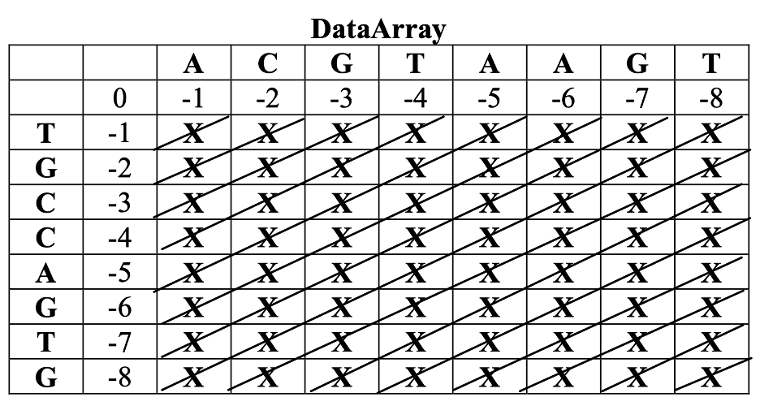
\includegraphics{Figures/8.png}}}
\caption{Sections that can be calculated in parallel. \cite{naveed_siddiqui_ahmed}}
\label{8}
\end{figure}

The limitation of this method is that the parallelization can be done only within each anti-diagonal. To start filling in the next anti-diagonal, the preceding anti-diagonal must already be all completed. Otherwise, there would not be enough information to calculate all of the scores for that anti-diagonal. The scores in each anti-diagonal is dependent on the scores in the preceding anti-diagonal.

According to the authors, the parallel version of the Needleman-Wunsch algorithm has a runtime of O(N+M) \cite{naveed_siddiqui_ahmed}. This is an improvement over the O(MN) runtime of the original algorithm.

\section*{Appendix}
\setcounter{section}{0}

\section{Current Progress}

At this point in the project, we have thoroughly researched the main algorithms used for sequence alignment and are able to follow and understand them pretty well. We have been able to implement the sequential versions of these algorithms in Java and have them compile and output correctly. We are currently experimenting with implementing parallelized versions of the algorithms.
 
We did face some challenges along the way. For instance, during our first attempt to parallelize the Needleman-Wunsch algorithm using the anti-diagonal technique, we were able to get the code to compile and output correctly. The runtime, however, was much worse than that of the sequential version. This was due to the way in which we were creating new threads. We were creating the threads inside a loop. We did this in an attempt to have those threads only process the current anti-diagonal. This constant spawning of new threads each iteration, however, caused a major slowdown. We were able to fix this by moving the thread creation outside the loop. We then used a spin wait to prevent the next anti-diagonal from being processed prematurely.
 
Our next step for the project is to keep on experimenting and trying known techniques to improve on efficiency. For example, we will attempt to make our implementations non-blocking. We will also start writing down our experiments and results and add to the report. Our final goal is to possibly venture out and try some of the newer methods out there. For instance, there are implementations out there that use GPU acceleration to help with parallelization. We could possibly head in that direction.

\bibliographystyle{IEEEtran}
\bibliography{IEEEabrv,References}

\end{document}